\label{Chapter:Design and Procedure of the User Study}
\section{Hypotheses}
\label{section DPUS: Hypotheses}
In Chapter \ref{Chapter:Automated Guided Jumping} we looked at a technique for automated guided navigation using the jumping metaphor and we also saw how the jumps in this technique could be made comprehensible so that the user would know when and where they will jump. The motivations and scenarios that might require such a technique were discussed in Chapter \ref{Chapter:Guided Jumping Motivation}. Keeping in mind the motivation to have a virtual museum that novice \acrshort{vr} users are able to explore we came up with the research questions \cref{rq:rq1}, \cref{rq:rq2} and \cref{rq:rq3} that are mentioned in section \ref{section GJM: Conclusion}.

To study the developed technique with regards to these research questions we decided to design a study that would compare our developed technique for automated guided jumping with a user controlled (free) jumping technique having visual guidance. With this study we hoped to prove the following hypotheses:

\begin{hypothesis}
	\label{hyp:hyp1}
	Participants do not get more simulator sickness while using the automated guided jumping compared to free jumping with visual guidance.
\end{hypothesis}
\begin{hypothesis}
	\label{hyp:hyp2}
	Visual previews before automated jumps will have similar comprehensibility of the jumps compared to free jumping with visual guidance.
\end{hypothesis}
\begin{hypothesis}
	\label{hyp:hyp3}
	Automated guided jumping will reduce task load compared to free jumping with visual guidance.
\end{hypothesis}
\begin{hypothesis}
	\label{hyp:hyp4}
	Users will be able to recall their path when using automated guided jumping as well as when free jumping with visual guidance.
\end{hypothesis}

Hypothesis \cref{hyp:hyp1} is important because we want to justify the need for automate the guided jumping without compromising on the reason for using jumping as the navigation metaphor, that is reduced motion sickness. To also justify that spatial awareness is similar in our technique versus free jumping the study must prove hypothesis \cref{hyp:hyp2} and \cref{hyp:hyp4}. Hypothesis \cref{hyp:hyp2}  also needs to be proved to show that the technique is easy to understand and users will not get confused when using it compared to free jumping. In order to prove the benefit of automated guided jumping over free jumping with visual guidance the study must show that \cref{hyp:hyp3} is true.  

\section{Study Task and Limitations}
\label{section DPUS: Study Task and Limitations}
As the study will be comparing automated jumping with free jumping using visual guiding, it was important to plan a controlled study design such that there would be no other influencing variables besides the automation. Therefore, when developing the free jumping technique that would be used for comparison we had to make sure that the only difference between it and our automated jumping technique would be that the user would make the jumps themselves instead of being automatically moved. There are still nodes and way points in the scene that are used to show visual guidance with an avatar being visible at the next node and a path drawn through way points as in figure \ref{fig:study-free-jumping}. The figure also shows the teleportation indicator with a curve pointing to it that users can use to select the position and orientation they want to be at after the jump.

\begin{figure}[]
	(\centering 1)
	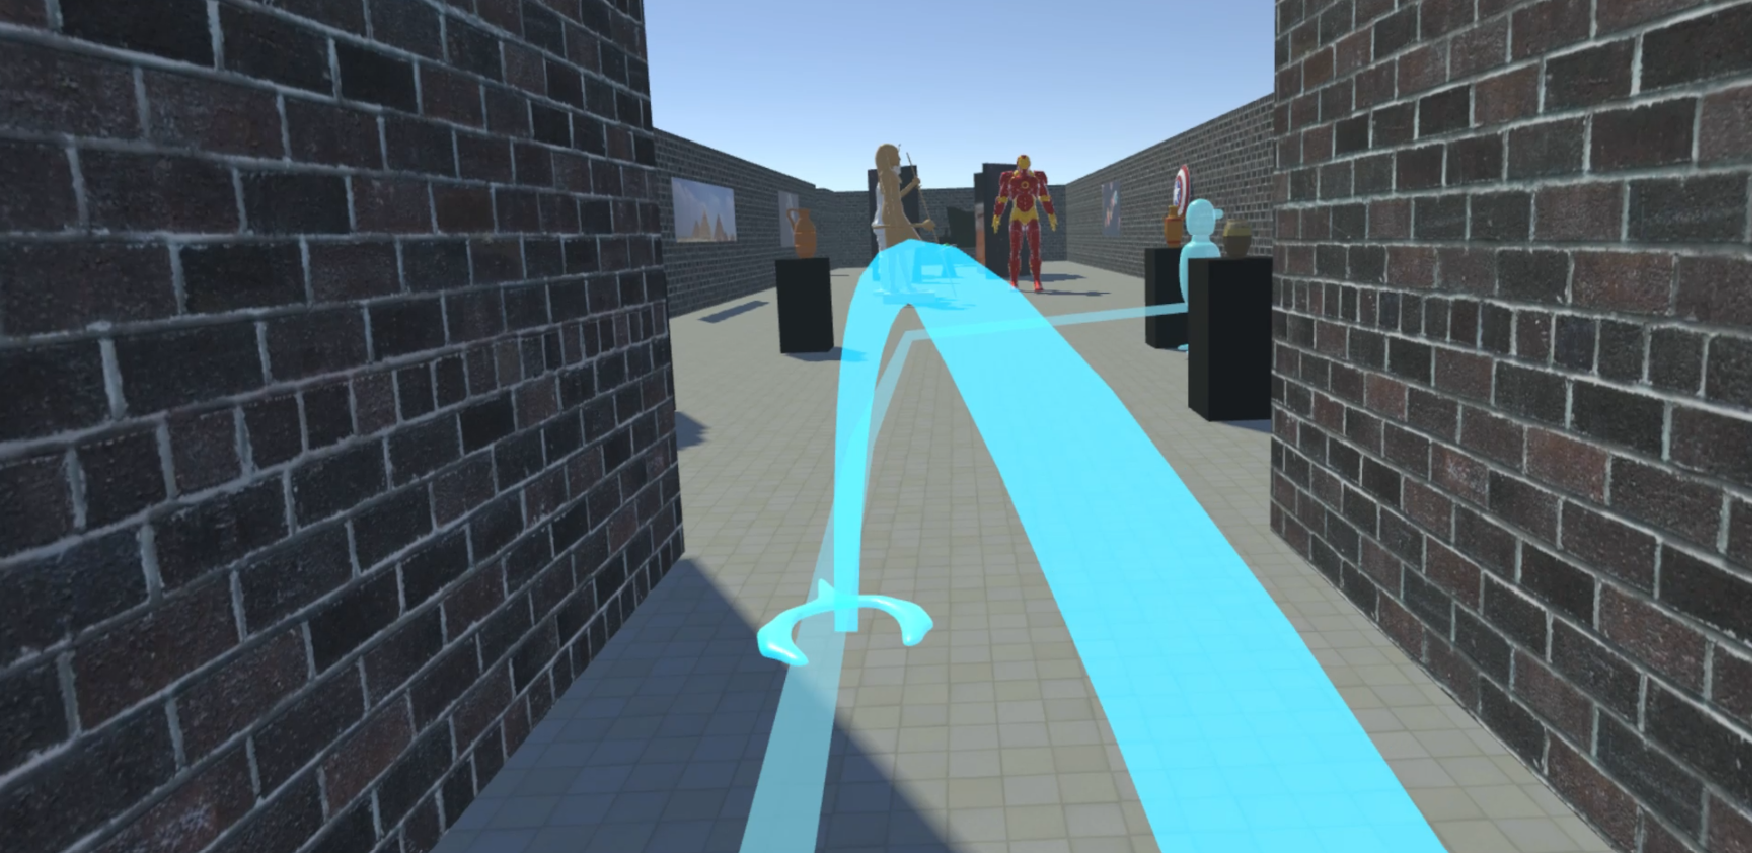
\includegraphics[width=0.25\textwidth]{images/free-jumping.pdf}
	(\centering 2)
	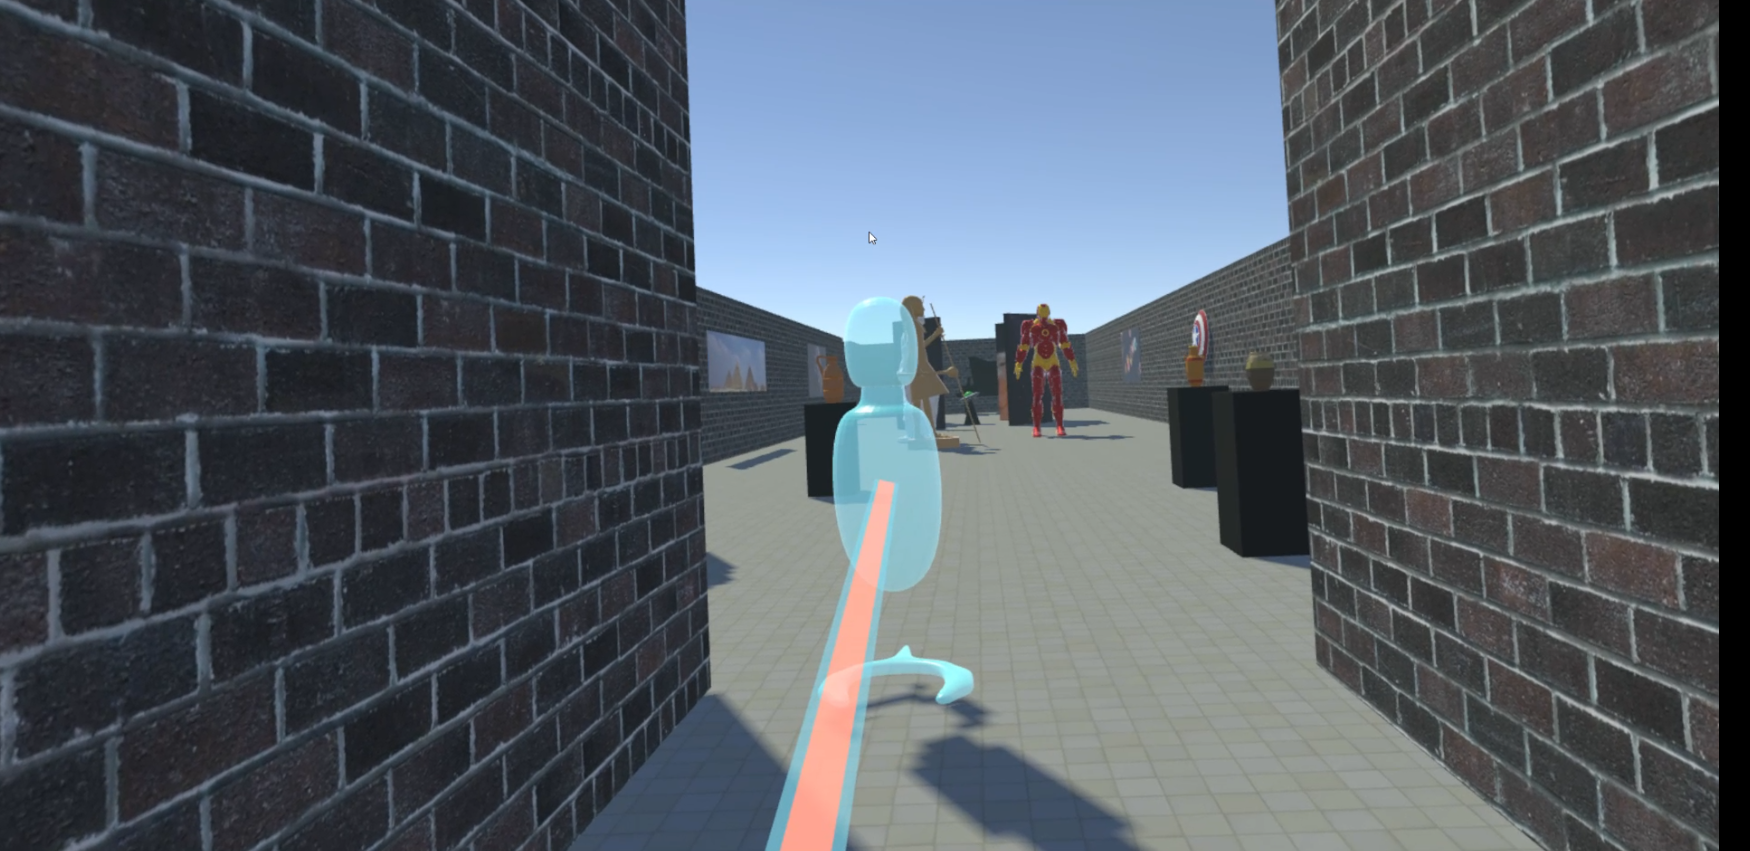
\includegraphics[width=0.25\textwidth]{images/automated-jumping.pdf}
	\caption{Free jumping with visual guidance.}
	\label{fig:study-free-jumping}
\end{figure}

As discussed in \ref{section GJM: Virtual Tours} one of the use cases for guiding techniques is virtual tours and we developed our technique for such a scenario as mentioned in section \ref{subsection AGJ ID: Scenario}. Therefore, the study design also kept in mind a virtual tour situation and considered the potential problem situations that may occur and the possible tasks that may be expected when touring through a virtual space. For this study the task was narrowed to touring a virtual museum with exhibits and trying to remember the path taken as well as the objects seen. This is a useful task when going through a museum and gives answers about whether the techniques used are facilitating acquisition of relevant knowledge of the scene as we hoped to do so through our technique and can be seen in our research question \cref{rq:rq1}.

This task situation for this study will not cover all possible situations that may arise when taking a virtual tour such as:
\begin{itemize}
	\item Exhibits that are very close or far from each other.
	\item More than 2 possible paths to choose from at some nodes.
\end{itemize} 

\section{Variables and Conditions}
\label{section DPUS: Variables and Conditions}
Keeping in mind the task of touring a museum and remembering the path and objects, there are certain variables that need to be varied between the two techniques and others that need to be measured. 

\subsection{Independent Variables}
\label{subsection DPUS VC: Independent Variables}
As we saw in section \ref{section DPUS: Study Task and Limitations}, automation is the only variable that should be different between the two techniques that are being compared. This means that one technique will have automated jumping and the other will not but the visual guidance and ability to have a choice must remain the same. In addition it is important to keep the number of nodes and way points the same. It is also necessary to keep the environment and objects of similar complexity. 

\subsection{Dependent Variables}
\label{subsection DPUS VC: Dependent Variables}
The variables that would depend on whether the technique is automated or not are related to the hypothesis that we introduced in section \ref{section DPUS: Hypotheses}. The amount of simulator sickness needs to be measured somehow to answer hypothesis \cref{hyp:hyp1}. A higher amount of simulator sickness is undesirable while lower amounts are better. Hypotheses \cref{hyp:hyp2} can only be answered by finding some way to determine comprehensibility of jumps.

\subsection{Study Conditions}
\label{subsection DPUS VC: Study Conditions}

\section{Study Procedure}
\label{section DPUS: Study Procedure}
In the previous section we defined variables and conditions for the study. Based on these we planned the study procedure which we will now outline in this section starting with the study setup followed by the study plan.

\subsection{Study Setup}
\label{subsection DPUS SP: Study Setup}

\subsection{Study Plan}
\label{subsection DPUS SP: Study Plan}

\section{Conclusion}
\label{section DPUS: Conclusion}



